\documentclass{tufte-book}

\hypersetup{colorlinks}% uncomment this line if you prefer colored hyperlinks (e.g., for onscreen viewing)

%%
% Book metadata
\title{Mathematical Methods for Engineers}
\author[CAPT Stu Blair]{United States Naval Academy}
\publisher{Mighty Goat Press}

%%
% If they're installed, use Bergamo and Chantilly from www.fontsite.com.
% They're clones of Bembo and Gill Sans, respectively.
%\IfFileExists{bergamo.sty}{\usepackage[osf]{bergamo}}{}% Bembo
%\IfFileExists{chantill.sty}{\usepackage{chantill}}{}% Gill Sans

%\usepackage{microtype}

%%
% Just some sample text
\usepackage{lipsum}

%%
% For nicely typeset tabular material
\usepackage{tabularx}
\usepackage{booktabs}

%%
% For graphics / images
\usepackage{graphicx}
\setkeys{Gin}{width=\linewidth,totalheight=\textheight,keepaspectratio}
\graphicspath{{graphics/}}

% The fancyvrb package lets us customize the formatting of verbatim
% environments.  We use a slightly smaller font.
\usepackage{fancyvrb}
\fvset{fontsize=\normalsize}

%%
% Prints argument within hanging parentheses (i.e., parentheses that take
% up no horizontal space).  Useful in tabular environments.
\newcommand{\hangp}[1]{\makebox[0pt][r]{(}#1\makebox[0pt][l]{)}}

%%
% Prints an asterisk that takes up no horizontal space.
% Useful in tabular environments.
\newcommand{\hangstar}{\makebox[0pt][l]{*}}

%%
% Prints a trailing space in a smart way.
\usepackage{xspace}

%%%% packages added by Stu

\usepackage{comment}

% fancy enumeration tricks
\usepackage{enumitem}

% have appendices
\usepackage{appendix}

% has sfrac command
\usepackage{xfrac}

% mathtools for over/under brace/bracket among other nifty tools
\usepackage{mathtools}


\usepackage{cancel} % to get oblique strike-through

%\usepackage{minted}
\usepackage{pifont}
\usepackage{color}

\usepackage{listings}
\definecolor{mygreen}{rgb}{0,0.6,0}
\definecolor{mygray}{rgb}{0.5,0.5,0.5}
\definecolor{mymauve}{rgb}{0.58,0,0.82}
\lstset{ %
  backgroundcolor=\color{white},   % choose the background color; you must add \usepackage{color} or \usepackage{xcolor}
  basicstyle=\footnotesize,        % the size of the fonts that are used for the code
  breakatwhitespace=false,         % sets if automatic breaks should only happen at whitespace
  breaklines=true,                 % sets automatic line breaking
  captionpos=b,                    % sets the caption-position to bottom
  commentstyle=\color{mygreen},    % comment style
  deletekeywords={...},            % if you want to delete keywords from the given language
  escapeinside={\%*}{*)},          % if you want to add LaTeX within your code
  extendedchars=true,              % lets you use non-ASCII characters; for 8-bits encodings only, does not work with UTF-8
  frame=single,                    % adds a frame around the code
  inputpath=./matlab_examples/,
  keepspaces=true,                 % keeps spaces in text, useful for keeping indentation of code (possibly needs columns=flexible)
  keywordstyle=\color{blue},       % keyword style
  language=Matlab,                 % the language of the code
  morekeywords={*,...},            % if you want to add more keywords to the set
  numbers=left,                    % where to put the line-numbers; possible values are (none, left, right)
  numbersep=5pt,                   % how far the line-numbers are from the code
  numberstyle=\tiny\color{mygray}, % the style that is used for the line-numbers
  rulecolor=\color{black},         % if not set, the frame-color may be changed on line-breaks within not-black text (e.g. comments (green here))
  showspaces=false,                % show spaces everywhere adding particular underscores; it overrides 'showstringspaces'
  showstringspaces=false,          % underline spaces within strings only
  showtabs=false,                  % show tabs within strings adding particular underscores
  stepnumber=2,                    % the step between two line-numbers. If it's 1, each line will be numbered
  stringstyle=\color{mymauve},     % string literal style
  tabsize=2,                       % sets default tabsize to 2 spaces
  title=\lstname                   % show the filename of files included with \lstinputlisting; also try caption instead of title
}

% example usage for code: \begin{lstlisting}[caption=< caption text >, label=<label>]

%%% end packages added by Stu
%%
% Some shortcuts for Tufte's book titles.  The lowercase commands will
% produce the initials of the book title in italics.  The all-caps commands
% will print out the full title of the book in italics.
\newcommand{\vdqi}{\textit{VDQI}\xspace}
\newcommand{\ei}{\textit{EI}\xspace}
\newcommand{\ve}{\textit{VE}\xspace}
\newcommand{\be}{\textit{BE}\xspace}
\newcommand{\VDQI}{\textit{The Visual Display of Quantitative Information}\xspace}
\newcommand{\EI}{\textit{Envisioning Information}\xspace}
\newcommand{\VE}{\textit{Visual Explanations}\xspace}
\newcommand{\BE}{\textit{Beautiful Evidence}\xspace}

\newcommand{\TL}{Tufte-\LaTeX\xspace}

% Prints the month name (e.g., January) and the year (e.g., 2008)
\newcommand{\monthyear}{%
  \ifcase\month\or January\or February\or March\or April\or May\or June\or
  July\or August\or September\or October\or November\or
  December\fi\space\number\year
}


% Prints an epigraph and speaker in sans serif, all-caps type.
\newcommand{\openepigraph}[2]{%
  %\sffamily\fontsize{14}{16}\selectfont
  \begin{fullwidth}
  \sffamily\large
  \begin{doublespace}
  \noindent\allcaps{#1}\\% epigraph
  \noindent\allcaps{#2}% author
  \end{doublespace}
  \end{fullwidth}
}

% Inserts a blank page
\newcommand{\blankpage}{\newpage\hbox{}\thispagestyle{empty}\newpage}

\usepackage{units}

% Typesets the font size, leading, and measure in the form of 10/12x26 pc.
\newcommand{\measure}[3]{#1/#2$\times$\unit[#3]{pc}}

% Macros for typesetting the documentation
\newcommand{\hlred}[1]{\textcolor{Maroon}{#1}}% prints in red
\newcommand{\hangleft}[1]{\makebox[0pt][r]{#1}}
\newcommand{\hairsp}{\hspace{1pt}}% hair space
\newcommand{\hquad}{\hskip0.5em\relax}% half quad space
\newcommand{\TODO}{\textcolor{red}{\bf TODO!}\xspace}
\newcommand{\na}{\quad--}% used in tables for N/A cells
\providecommand{\XeLaTeX}{X\lower.5ex\hbox{\kern-0.15em\reflectbox{E}}\kern-0.1em\LaTeX}
\newcommand{\tXeLaTeX}{\XeLaTeX\index{XeLaTeX@\protect\XeLaTeX}}
% \index{\texttt{\textbackslash xyz}@\hangleft{\texttt{\textbackslash}}\texttt{xyz}}
\newcommand{\tuftebs}{\symbol{'134}}% a backslash in tt type in OT1/T1
\newcommand{\doccmdnoindex}[2][]{\texttt{\tuftebs#2}}% command name -- adds backslash automatically (and doesn't add cmd to the index)
\newcommand{\doccmddef}[2][]{%
  \hlred{\texttt{\tuftebs#2}}\label{cmd:#2}%
  \ifthenelse{\isempty{#1}}%
    {% add the command to the index
      \index{#2 command@\protect\hangleft{\texttt{\tuftebs}}\texttt{#2}}% command name
    }%
    {% add the command and package to the index
      \index{#2 command@\protect\hangleft{\texttt{\tuftebs}}\texttt{#2} (\texttt{#1} package)}% command name
      \index{#1 package@\texttt{#1} package}\index{packages!#1@\texttt{#1}}% package name
    }%
}% command name -- adds backslash automaticallygit@github.com:stu314159/Nuclear_Plant_Engineering.git
\newcommand{\doccmd}[2][]{%
  \texttt{\tuftebs#2}%
  \ifthenelse{\isempty{#1}}%
    {% add the command to the index
      \index{#2 command@\protect\hangleft{\texttt{\tuftebs}}\texttt{#2}}% command name
    }%
    {% add the command and package to the index
      \index{#2 command@\protect\hangleft{\texttt{\tuftebs}}\texttt{#2} (\texttt{#1} package)}% command name
      \index{#1 package@\texttt{#1} package}\index{packages!#1@\texttt{#1}}% package name
    }%
}% command name -- adds backslash automatically
\newcommand{\docopt}[1]{\ensuremath{\langle}\textrm{\textit{#1}}\ensuremath{\rangle}}% optional command argument
\newcommand{\docarg}[1]{\textrm{\textit{#1}}}% (required) command argument
\newenvironment{docspec}{\begin{quotation}\ttfamily\parskip0pt\parindent0pt\ignorespaces}{\end{quotation}}% command specification environment
\newcommand{\docenv}[1]{\texttt{#1}\index{#1 environment@\texttt{#1} environment}\index{environments!#1@\texttt{#1}}}% environment name
\newcommand{\docenvdef}[1]{\hlred{\texttt{#1}}\label{env:#1}\index{#1 environment@\texttt{#1} environment}\index{environments!#1@\texttt{#1}}}% environment name
\newcommand{\docpkg}[1]{\texttt{#1}\index{#1 package@\texttt{#1} package}\index{packages!#1@\texttt{#1}}}% package name
\newcommand{\doccls}[1]{\texttt{#1}}% document class name
\newcommand{\docclsopt}[1]{\texttt{#1}\index{#1 class option@\texttt{#1} class option}\index{class options!#1@\texttt{#1}}}% document class option name
\newcommand{\docclsoptdef}[1]{\hlred{\texttt{#1}}\label{clsopt:#1}\index{#1 class option@\texttt{#1} class option}\index{class options!#1@\texttt{#1}}}% document class option name defined
\newcommand{\docmsg}[2]{\bigskip\begin{fullwidth}\noindent\ttfamily#1\end{fullwidth}\medskip\par\noindent#2}
\newcommand{\docfilehook}[2]{\texttt{#1}\index{file hooks!#2}\index{#1@\texttt{#1}}}
\newcommand{\doccounter}[1]{\texttt{#1}\index{#1 counter@\texttt{#1} counter}}

% Generates the index
\usepackage{makeidx}
\makeindex

\begin{document}

\begin{fullwidth}
\thispagestyle{empty}
\begin{figure}
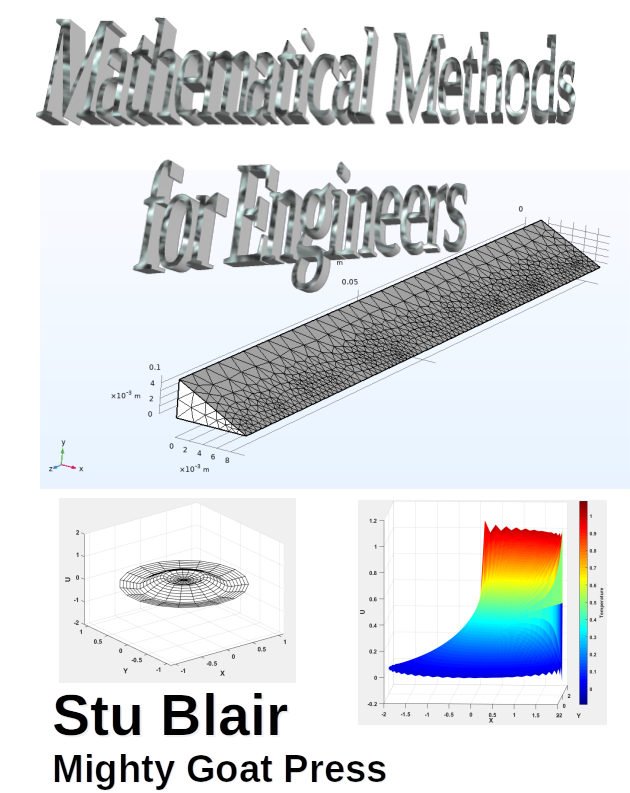
\includegraphics[width=1.5\textwidth]{cover1.png}
\end{figure}
\end{fullwidth}

% Front matter
\frontmatter

% r.1 blank page
%\blankpage


% v.2 epigraphs
\newpage\thispagestyle{empty}
\vfill
\openepigraph{%
The only way to learn mathematics is to do mathematics.
}{P.R. Halmos}

\vfill
\openepigraph{%
The purpose of computing is insight, not pictures
}{L.N. Trefethen}


\vfill
\openepigraph{%
Never do a calculation until you already know the answer.
}{J.A. Wheeler}


% r.3 full title page
\maketitle


% v.4 copyright page
\newpage
\begin{fullwidth}
~\vfill
\thispagestyle{empty}
\setlength{\parindent}{0pt}
\setlength{\parskip}{\baselineskip}
Copyright \copyright\ \the\year\ \thanklessauthor
\par\smallcaps{Published by \thanklesspublisher}

%\par\smallcaps{tufte-latex.github.io/tufte-latex/}
%
%\par Licensed under the Apache License, Version 2.0 (the ``License''); you may not
%use this file except in compliance with the License. You may obtain a copy
%of the License at \url{http://www.apache.org/licenses/LICENSE-2.0}. Unless
%required by applicable law or agreed to in writing, software distributed
%under the License is distributed on an \smallcaps{``AS IS'' BASIS, WITHOUT
%WARRANTIES OR CONDITIONS OF ANY KIND}, either express or implied. See the
%License for the specific language governing permissions and limitations
%under the License.\index{license}

\par\textit{First printing, \monthyear}
\end{fullwidth}

% r.5 contents
\tableofcontents

\listoffigures

\listoftables

% r.7 dedication
%\cleardoublepage
%~\vfill
%\begin{doublespace}
%\noindent\fontsize{18}{22}\selectfont\itshape
%\nohyphenation
%Dedicated to the midshipmen of the United States Naval Academy; the future of our armed services and of %our country.
%\end{doublespace}
%\vfill
%\vfill


% r.9 introduction
\cleardoublepage
\chapter*{Preface}

The purpose of this text is to provide a concise reference for engineering students who would like to strengthen their conceptual understanding and practical proficiency in analytical and numerical methods in engineering.  The material is based on a sequence of two courses taught at the United States Naval Academy.  

\subsection*{Analytical Methods}

The first course focused on analytical methods for linear ordinary and partial differential equations.  All students came into the course having taken a three-semester sequence of calculus along with a course in ordinary differential equations.  The analytical methods portion quickly reviews methods for constant coefficient linear equations and proceeds to methods for non-constant coefficients including Cauchy-Euler equations, power series methods, and method of Frobenieus.  After a review of Fourier Series methods and an introduction to Fourier-Legendre and Fourier-Bessel expansions we thoroughly explore solutions to second-order, linear, partial differential equations.  Since many students are also studying nuclear engineering, there is a heavy focus on addressing boundary value problems in cylindrical and spherical coordinate systems that are applicable to other topics of interest such as reactor physics.  There is also heavy emphasis on heat transfer applications that students will see later on in their undergraduate curriculum.

The materials presented are based heavily on Professor Dennis Zill's excellent book.\cite[-3cm]{zill2020advanced} We lightly select from chapters 1-3 for review; chapter 5 for series solution methods; and chapters 12-14 for Fourier Series and solutions to linear boundary value problems.  Material from that text is used throughout this book.  

What distinguishes this course from Prof Zill's work is the incorporation of computational tools in the solution process.  These ``semi-analytical methods'' are presented here in MATLAB\cite[-3.75cm]{matlab} owing to the students preparation with that tool.  Other open-source tools like Octave\cite[-3.5cm]{octave} and Python,\cite[-1cm]{10.5555/1593511} of course, could be used. 

\subsection*{Numerical Methods}

%%
% Start the main matter (normal chapters)
\mainmatter

\part{Introduction and Review}

\chapter{Lecture 1 - Course Introduction and Numeric Preliminaries}
\label{ch:lec1n}
\section{Objectives}
The objectives of this lecture are:
\begin{itemize}
\item Introduce the course objectives.
\item Describe how numbers are represented on computers.
\item Outline sources of errors in numerical methods relative to analytical methods.
\end{itemize}
\setcounter{lstannotation}{0}

\section{Course Introduction}

This course is intended to be an introduction and overview of numerical methods.\marginnote[-0.5cm]{\textbf{Question:} What are numerical methods? 

\vspace{0.25cm}

\noindent \textbf{Answer:} Numerical methods (or numerical analysis) is the study of \emph{algorithms} for the problems of \emph{continuous} mathematics.}  The target audience comprises undergraduate students of engineering who have already taken a full sequence of calculus and differential equations courses.  Some students may also have taken the analytical methods course described earlier in this book. All students are expected to have some proficiency in the MATLAB programming environment.  

\subsection{Objectives}
\newthought{The objectives} for this course are as follows:

\begin{enumerate}
\item Students will understand the fundamentals of numerical methods with an emphasis on the most essential algorithms and methods.

\item Students will have enhanced their scientific computing skills and further developed their proficiency in using the MATLAB environment to implement algorithms and have learned to critically evaluate their results.

\item Students will understand the fundamentals of the finite element method (FEM) and have attained an introductory-level proficiency in using the COMSOL software package to carry out a multi-physics analysis of a relevant physical model.

\item Students will have developed the ability to formulate a problem of interest, apply numerical methods and computational tools to analyze the problem, and communicate pertinent results to others.
\end{enumerate}


\subsection{Course Topics}
The specific topics we will cover include:

\begin{enumerate}
\item Methods for solving non-linear equations
\begin{enumerate}
\item Bisection method
\item Newton's method
\item Secant method

\end{enumerate}
\item Methods for solving linear equations
\begin{enumerate}
\item Gauss elimination and related methods like LU- and Cholesky factorization
\item Iterative solution methods for sparse linear systems of equations\sidenote{We will also discuss some preconditioners.}
\end{enumerate}
\item Curve fitting
\begin{enumerate}
\item Least squares algorithms
\item Curve fitting with Lagrange polynomials
\end{enumerate}
\item Numeric differentiation
\begin{enumerate}
\item Finite difference methods
\item Lagrange polynomials
\end{enumerate}
\item Numeric integration
\begin{enumerate}
\item A variety of Newton-Cotes methods
\item Gauss Quadrature
\end{enumerate}

\item Initial- and Boundary-value problems \sidenote{This section will prominently include MATLAB built-in methods; particularly for boundary value problems.}
\begin{enumerate}
\item Runge-Kutta methods for initial value problems\sidenote{We will not extensively cover either explicit or implicit multi-step methods, giving preference to the wide variety of very effective RK methods.}
\item Shooting method for boundary value problems
\item Finite element method\sidenote{There will be a simple MATLAB demonstration with application to one-dimensional boundary value problems.  The majority of FEM coverage will be related to the use of COMSOL.}
\end{enumerate}

\end{enumerate}  

\vspace{4.0cm}

\section{Representation of Numbers on a Computer}

Every engineer who uses computational tools in their work should have a basic understanding of how numbers are represented on a computer.  The essential take-aways from this section are:
\begin{enumerate}
\item Since the computer is a finite machine, only a finite set of numbers can be exactly represented on the computer.  All other numbers are approximated.
\item Computers store integers and non-integers differently and the limits to what numbers can be represented or how exactly they are represented are also different.
\item The fact that numbers, in general, are represented inexactly on the computer has an impact on how algorithms are developed.
\end{enumerate}

\subsection{Integers}
Integers are represented exactly on a computer, but only a finite subset of all integers can be represented.  There are a number of integer types that are supported by common computer architectures and language compilers.\marginnote[-4.5cm]{Some of the integer data types specified by the C++ language standard include:
\begin{enumerate}
\item signed char (8 bits)
\item short int (16 bits)
\item int (at least 16 bits -- usually 32 bits)
\item long int (at least 32 bits)
\item long long int (at least 64 bits)
\end{enumerate}
Each of these categories includes a signed and unsigned variant.  Even within these categories there is fuzziness---e.g. \emph{``at least 16 bits''}---that allows for variations between different compiler implementations and computer hardware (e.g. Intel vs. AMD CPU).
}\marginnote{\textbf{Note:} The word \emph{bit} is taken to be synonymous with the words \emph{binary digit}.} For the purposes of this class we will focus on two types: \emph{unsigned integers} and \emph{signed integers}.  To further focus the discussion we will only consider 32-bit representations of signed and unsigned integers.

\newthought{Perhaps the easiest} integer representation to understand is the 32-bit unsigned integer.\sidenote{You can create a 32-bit unsigned integer in MATLAB by typing:

\vspace{0.1cm}

\noindent \lstinline[style=myMatlab]{x = uint32(1994)}

\vspace{0.1cm}

Variables with other data types can be constructed using similar syntax; see the MATLAB documentation for details.
} In this format 32 binary digits corresponding to $2^0$ to $2^{31}$ are stored in memory.  Numbers in binary work the same way our normal decimal number work: just base 2 instead of base 10.  For example, the 32-bit unsigned integer representation of the number 23 is shown in Figure \ref{fig:lec1n-binary-23}.


\begin{figure}[h!]
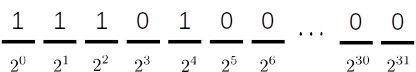
\includegraphics[width=0.75\columnwidth]{binary_23.png}
\caption{The number 23 in unsigned integer format.}
\label{fig:lec1n-binary-23}
\end{figure}


%\vspace{0.25cm}
%\noindent (image of 24 in binary)
%\vspace{0.25cm}

With 32-bit unsigned integers the computer can exactly represent all integers between 0 and $2^{32}-1$. Negative integers and integers greater than $2^{31}$ are not represented at all.%\sidenote{\textbf{Question:} What do you get from the following MATLAB code?
%\begin{lstlisting}[style=myMatlab]
%a = uint32(2^32-1);
%b = uint32(1);
%c = a + b;
%fprintf('c = %d \n',c);
%\end{lstlisting}

%\lstinline[style=myMatlab]{ a = uint32(2^32 - 1)  b = unit32(1) }

%\vspace{0.1cm}

%\noindent\textbf{Answer:} The variable c will still be equal to $2^{31}-1$.  MATLAB will round numbers outside of the range of representation for 32-bit unsigned ints to the nearest endpoint which, in this case, is $2^{31}-1$.
%}

\newthought{There are fewer} applications for which \emph{signed integers} will be used for this course, but they are, naturally, important.  Perhaps the most obvious way that a computer might represent signed integers would be to just use the same format as unsigned integers except to reserve one bit for the sign.  This is not, however, the way it is normally done.  For one thing, this approach results in there being two different bit-patterns for zero.  This might seem like a trivial inconvenience but it is not the sort of thing that passes without notice in computer engineering circles. Another, perhaps more significant, issue with this approach is that special logic would be needed when adding or subtracting a mixture of positive and negative integers. (i.e. you would not be able to use the same circuitry on the microprocessor for adding positive and negative numbers together as you would for adding two positive numbers.)
  
The format that is normally used today for representing signed integers is called \emph{two's complement}.  If you want to write a positive number in two's complement format, you do the same thing as you would normally do for an unsigned integer.\sidenote[][-1.5cm]{Except, as it turns out, the largest positive 32-bit signed integer will only half as large as the corresponding largest signed integer.} If you need to write a negative number, you start by expressing the positive number, then you \emph{take the complement of each binary digit} and, when you are done with that, you \emph{add one.} A demonstration of this number representation, shortened to 5-bits to make it more compact, is shown in Figure \ref{fig:twos-complement-demo}.  


\begin{marginfigure}
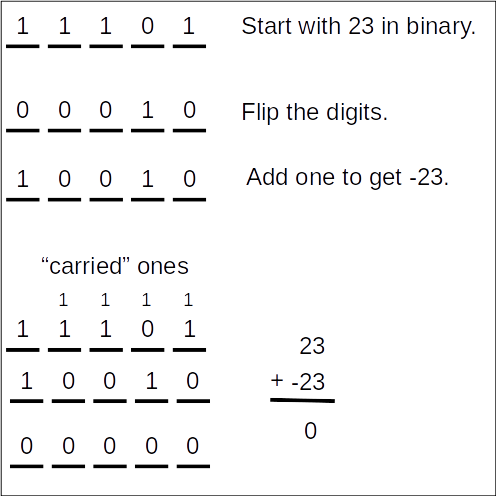
\includegraphics{twos-complement-demo.png}
\caption{Demonstration of twos-complement: adding 23 and -23 in 5-bit representation.}
\label{fig:twos-complement-demo}
\end{marginfigure}

%\vspace{0.25cm}
%\noindent (image showing example two's complement)
%\vspace{0.25cm}

This representation has the advantages that: a) there is only a single representation for zero; and b) the same hardware is used for both addition and subtraction (i.e. to subtract you simply add a negative number.)

\subsection{Floating Point Numbers}
In general, binary floating point numbers are given in the form shown in Equation \ref{eq:bfpn-format}:
\begin{equation}
1.\underbrace{\text{fff}\dots\text{f}}_{\text{mantissa}} \times 2^{\underbrace{\text{eee}\dots\text{e}}_{\text{exponent}}}
\label{eq:bfpn-format}
\end{equation}
where a number of digits available are divided between the fraction, or \emph{mantissa}, and \emph{exponent}.  In any finite machine, there will be a limit to the number of total digits available.  Thus an engineering decision needs to be made to determine how many digits will be allocated to the mantissa and how many for the exponent.  If you have more digits in the mantissa, you will be able to represent numbers that are closer together---the \emph{precision} of your representation will increase.  If you allocate more digits to the exponent, you will be able to represent numbers that are larger (for large positive exponents) or smaller (large negative exponents)---the \emph{range} of your representation will be wider.  The implications of these decisions should be clear: if you devote fewer bits to the mantissa, there will be more rounding errors in your calculations as real numbers are mapped, in some way, to the best floating point representation; if you devote fewer bits to the exponent, really large numbers and really small numbers will not be represented at all.  In earlier days of computing, different computer vendors made different decisions as to how floating point numbers would be represented.\cite{moler_fp1}  This caused problems when scientists tried to run the same code on different computers and got different results.  In 1985, the IEEE-754 standard was approved and, since then, has been adopted by essentially all computer manufacturers.  As a result, the menagerie of floating point formats and implementations have been tamed. Scientists and engineers could run their codes on different machines and expect to get the same results.

\begin{figure}
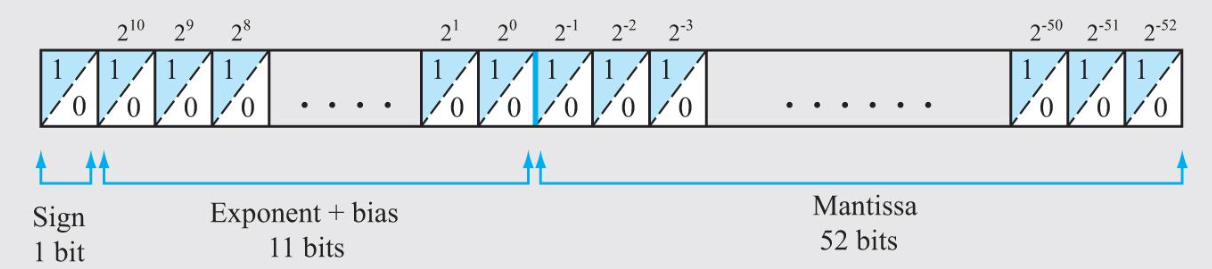
\includegraphics[width=0.94\columnwidth]{double-precision-format.png}
\caption{IEEE-754 double precision number format.}
\label{fig:double-precision-format}
\end{figure}

The IEEE-754 standard provides specification of several floating point number formats.  For this class, we will be concerned primarily with the \emph{double precision} floating point format which is illustrated in Figure \ref{fig:double-precision-format}.  This format uses a single sign bit (1 for negative, 0 for positive), 11 bits for the exponent which is encoded as an unsigned integer with bias,\sidenote{For double precision numbers, the bias is 1023.} and 52 bits for the mantissa.\sidenote{\textbf{Note:} The number 1 shown in Equation \ref{eq:bfpn-format} is not stored but is implicitly included in all \emph{normalized} floating point numbers.  This is done so that all numbers will have a \emph{unique} floating point representation. }  In the double precision format, the smallest positive number that can be represented is $2^{-1022}$ which is approximately equal to $2.2 \times 10^{-308}$.\marginnote{MATLAB includes built-in functions to report the smallest and largest representable floating point numbers.  The functions \lstinline[style=myMatlab]{realmin(precision)} and \lstinline[style=myMatlab]{realmax(precision)} will return the  smallest or largest positive floating point number for ``single'' or ``double'' precision floating point precision.} The smallest interval between numbers that can be represented is called \emph{machine epsilon}.\marginnote{In MATLAB, machine epsilon is provided with the function: \lstinline[style=myMatlab]{eps(precision)} for ``single'' and ``double'' precision.}  The size of this limit is driven by the number of bits in the mantissa.  For IEEE-754 double precision floating point numbers this is approximately $2.22 \times 10^{-16}$.\sidenote{Sometimes computational scientists refer to this as ``16 digits of precision.''}

\newthought{The procedure to} encode real numbers in the double precision floating point format will be illustrated with an example.

\vspace{0.5cm}

\noindent\textbf{Example:} Write the number -10.5 using the IEEE-754 double precision format.

\vspace{0.25cm}

\noindent\textbf{Step \#1:} Determine the mantissa and the exponent.  To do this, we normalize the number by dividing by $2^e$ where $e$ is the largest power of 2 that is \emph{less} than the magnitude of the number you are encoding.  

\vspace{0.1cm} 

\noindent In this case, $e=3$ since 10.5 is greater than $2^3$ but less than $2^4$.  

\begin{align*}
\frac{-10.5}{2^3} & = -1.3125 \\
\Rightarrow -10.5 &= -1.3125 \times 2^3
\end{align*}

\noindent Therefore the mantissa will need to encode 0.3215, and the exponent will need to encode 3 plus the bias of 1023, or 1026.

\vspace{0.25cm}

\noindent\textbf{Step \#2:} Set the sign bit. As the number is negative, the sign bit is: 1.

\vspace{0.25cm}


\noindent\textbf{Step \#3:} Calculate the 11 exponent bits.  

\begin{align*}
1026 &= 1024 + 2 \\
&= 1 \times 2^{10} + 1 \times 2^{1}
\end{align*}


\begin{figure}
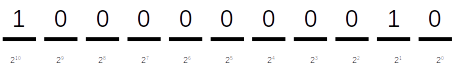
\includegraphics[width=0.75\columnwidth]{lec1n-ex1-exponent.png}
\caption{Exponent: 3+1023 = 1026 in 11-bit binary.}
\label{fig:lec1n-ex1-exponent}
\end{figure}   
  

\vspace{0.25cm}

\noindent\textbf{Step \#4:} Calculate the 52 mantissa bits to represent 0.3125.  The result is shown in Figure \ref{fig:lec1n-ex1-mantissa}.

\begin{figure}
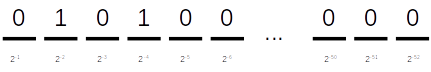
\includegraphics[width=0.75\columnwidth]{lec1n-ex1-mantissa.png}
\caption{Mantissa: 0.25 + 0.0625 = 0.3125.}
\label{fig:lec1n-ex1-mantissa}
\end{figure}

\noindent Where the calculations might be done as shown below:
\begin{align*}
0.3125 - 0 \times 2^{-1} &= 0.3125 \\
0.3125 - 1 \times 2^{-2} &= 0.0625 \\
0.0625 - 0 \times 2^{-3} &= 0.0625 \\
0.0625 - 1 \times 2^{-4} &= 0
\end{align*}
and all other entries are, of course, zero.


\section{Sources of Error} \index{error, truncation} \index{error, round-off} \index{error, modeling}

When using numerical methods there are several sources of error that you, as an engineer, should be aware of.  We have just discussed the details of double precision numbers so \emph{round-off error} is at the top of our mind.  Real numbers are not represented exactly on a computer but instead as floating point numbers.  The floating point number \emph{closest} to the real number gets used in its place. Error due to this round-off accumulates with mathematical operations.  Quantitative analysis of the accumulation of round-off-error is a tedious (albeit important) business that we will avoid in this class.  Nonetheless, engineers need to be aware that it is happening and, in a few instances, we will take steps to mitigate this build-up of error.

The second source of error that we will mention here is something that should be familiar to students who have taken the course in analytical methods: \emph{truncation error}.  In the analytical methods course we suffered from truncation error every time we shortened our infinite series solution to a finite number of terms.  We reduced this error by increasing the number of terms we retained, but there was no way to make it go away completely.  In this course we will see further instances of truncation error in most every algorithm we implement.  Derivatives and integrals that could, in principle, be done exactly, will be done approximately as we truncate the Taylor series expansion or limit the order of polynomials used to represent the exact derivative or integral.  We can reduce the magnitude of these errors, but we cannot make them go away entirely.

The third source of error mentioned here is \emph{modeling error}.  Modeling errors are reflected in the differences between observed physical phenomena and the corresponding mathematical model of the phenomena.  There are a couple of reasons for these differences and these include:
\begin{enumerate}
\item Linearization of non-linear processes.  Instances where you may already have done this, in your heat transfer or fluid dynamics class, include:
\begin{enumerate}
\item Assumption of constant thermal conductivity for heat conduction problems.  This assumption linearizes the heat equation and, for simple geometry, renders the problem amenable to analytical methods.  This assumption is retained for many numerical methods when solving the heat equation on more complex geometry.  The modeling error resulting from linearization remains.

\item Assumption of constant drag coefficient for external flow calculations.  Once again, this assumption simplifies the calculations at the cost of model fidelity.
\end{enumerate}

\item De-coupling of physical processes.  Nature does not specialize its behavior by academic subjects.  Consequently the air flowing over the control surfaces of a fighter jet is both a fluid dynamics and structural dynamics problem when the wing responds to forces imposed by the air.  Water flowing through a pressurized water reactor core is heated by forced convection and radiation that you might calculate in heat transfer class, but the resulting change in water properties also affect the neutron economy and power production rate that you might calculate in reactor physics which, in turn, will have further effect on the heat transfer problem.  We de-couple these processes so the analysis is more manageable but as a result the solution we arrive at is in error.  

\end{enumerate}  
Scientists and engineers need to be aware of all of these sources of errors and take steps to mitigate them where possible.






\part{Power Series Methods}


%%
% The back matter contains appendices, bibliographies, indices, glossaries, etc.

\part{Back Matter}
\backmatter

\bibliography{Mathematical_Methods_for_Engineers}
\bibliographystyle{plainnat}


\appendix
\appendixpage
\noappendicestocpagenum
\addappheadtotoc



\chapter{Matlab Style Rules}
\begin{enumerate}
\item \textbf{rule:} All scripts will start with the commands: \textbf{clear}, \textbf{clc}, and \textbf{close 'all'}

\textbf{rationale:} No script should depend upon any data visible in the MATLAB workspace when the script starts.  By omitting these commands, residual data within the workspace may hide errors.

\item \textbf{rule:} Your code must be documented with enough details such that a reader unfamiliar with your work will know what you are doing.

\textbf{rationale:} Code documentation is a habit. For more significant projects readers may need help in deciding what the author of the code intended.  For your own code, the most likely reader is you---a few months into the future.

\item \textbf{rule:} Function and variable names must be meaningful and reasonable in length.

\textbf{rationale:} Failing to do either make code harder to read and maintain.

\item \textbf{rule:} All outputs from the code \underline{\textbf{must}} be meaningful; numbers should be formatted, part of a sentence, and include units. Graphs should be readable and axis labels should make sense and include units.

\textbf{rationale:} Code output is a form of communication. It is important that this communication be clear and unambiguous.

\item \textbf{rule:} Do not leave warnings from the Code Analyzer unaddressed.

\textbf{rationale:} Sometimes Code Analyzer warnings can be safely ignored.  Most of the time the warning points to a stylistic error that would be unacceptable in software that you use. Occasionally these warnings are indicative of a hidden error.

\item \textbf{rule:} Use the ``smart indentation tool'' to format the indentation of your code.

\textbf{rationale:} This tool improves code readability. It will also occasionally point out errors that you did not see before.

\item \textbf{rule:} Pre-allocate arrays; if possible initialize with \textbf{NaN} values.

\textbf{rationale:} Pre-allocation improves performance and helps readability. Initialization with \textbf{NaN} helps avoid a range of potential logical errors.

\item \textbf{rule:} Avoid ``magic numbers'' --- i.e. hard-coded constants.

\textbf{rationale:} Constants included in your code tend to hide your program logic. Also, ``magic numbers'' make code maintenance more difficult and error prone.

\item \textbf{rule:} Only write one statement per line.

\textbf{rationale:} Multi-statement-lines hurt code readability in almost all cases.

\item \textbf{rule:} Do not write excessively long lines of code; use the line continuation ``...'' and indentation to spread long expressions over several lines.

\textbf{rationale:} Following this rule improves code readability.
\end{enumerate}


\printindex
\end{document}

